%!TEX root = thesis.tex

%time planning—having a Gantt chart is probably a better idea then just a list;

\chapter{Planning}
\label{chap:planning}

This chapter provides an overview of the deadlines for the thesis, ranging from the start of the thesis on November tenth, 2015 to the final deadline on June twentieth, 2016. Based on these deadlines a planning has been made, which breaks down the total workload into twelve parts. A GANTT chart is presented as a graphical presentation of the thesis planning. 

\section{Deadlines}
For the planning of the thesis a number of deadlines are import. At five moments in time the status of the thesis has to be presented and at three of these moments it is required to hand in a report. The five deadlines are referred to as P1 to P5 in the graduation manual. P1 took place on November tenth, 2015. The general idea for the thesis was presented here and a number of students and staff was present to provide feedback. This document is part of the deliverables for P2. At P2 the research proposal for the thesis needs to be handed in. This contains the research question, its relevance, a literature analysis of related work, a description of the methods, a planning and an overview of the tools and data that will be used. The research proposal is due January eleventh, 2016. The P2 presentation is scheduled on January eighteenth, 2016. Preliminary results are presented at P3, for which the date is still unknown. The P4 deadline is on May second, 2016. This is the deadline for handing in the first draft of the thesis report. It should also be presented on May seventh, 2016. The final deadline (P5) is on the thirteenth of June, 2016. The thesis outcomes will be presented on June twentieth, 2016.

\section{GANTT Chart}
\begin{figure}
	\centering
	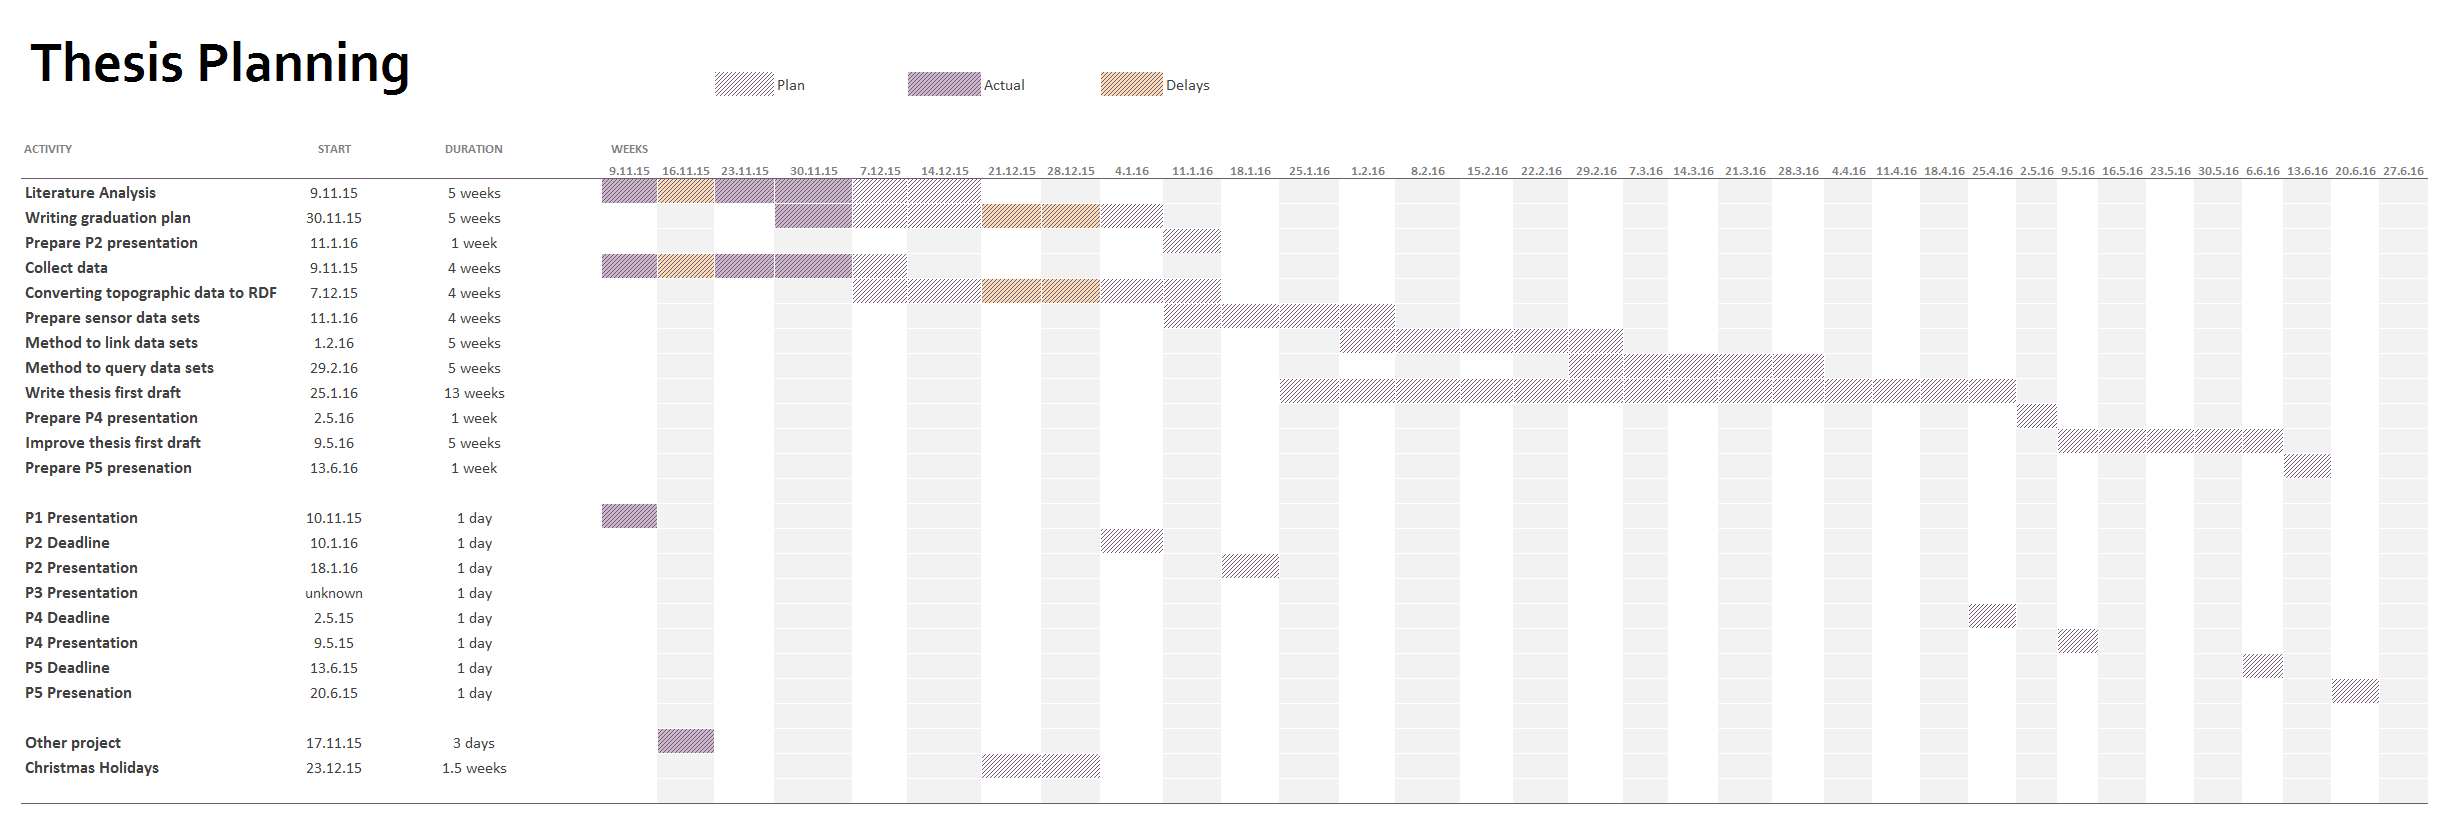
\includegraphics[width=2\linewidth, angle=90]{figs/GANTT-chart.png}
	\caption{GANTT chart showing the planning of the thesis}
	\label{fig:GANTT}
\end{figure}